\documentclass{article}
\usepackage{graphicx,datetime,hyperref,verbatim,caption,subcaption} % Required for inserting images

\usepackage{geometry}
\geometry{
a4paper,
total={170mm,257mm},
left=20mm,
top=20mm,
}

\newcommand{\setlasteditor}[1]{\gdef\lasteditor{#1}}
\newcommand{\lastedited}{%
    \vspace{1mm} {\footnotesize Last edited by: \lasteditor} \vspace{3mm}
    \newline

}

\title{ISTA ASTRO SOFTWARE}
\date{September 2024}

\begin{document}

\maketitle


\tableofcontents
\newpage
\section*{Introduction}
\setlasteditor{Aayush Desai}
\lastedited
\noindent
Hello world. This is the ISTA Software Page, which will hopefully have all the neat tools and tricks the department would have developed over the years. The repository is maintained by Aayush Desai for the time being, and is open to contributions from anyone who would like to add to it.
\newline
\noindent
Here you can find access to example scripts that are group agnostic (mostly). Should you have any ideas for further developments, just add another section and start writing.
\newline
\newline
For those working on Overleaf, once you are done with the edits, please make sure to push the changes to the repository. You can do this by:

\begin{enumerate}
    \item \textbf{Committing the changes:} This can be done by clicking on the "menu" button, on the top left corner of the screen, navigating to "github" and selecting commit changes. This will save the changes you have made to the repository.
    \item \textbf{Pushing the changes:} This can be done by clicking on the three dots on the top right corner of the screen, and selecting push changes. This will push the changes you have made to the repository.
    \item \textbf{Syncing the changes:} This can be done by clicking on the three dots on the top right corner of the screen, and selecting sync changes. This will sync the changes you have made to the repository.
\end{enumerate}
\noindent
For those working on the local machine, please make sure to:

\begin{enumerate}
    \item \textbf{Pull from the main repo} git pull from the repository to get the latest changes.
    \item \textbf{Make changed} make the changes you need to make.
    \item \textbf{Push to the main repo} git add, git commit, and git push the changes to the repository.
\end{enumerate}
\section{Sharing Repositories via GIT}
\setlasteditor{Aayush Desai}
\lastedited

\section{MESA on Cluster}
\setlasteditor{Lukas Einramhof}
\lastedited
IT has installed \texttt{MESA} on the cluster. In order to get \texttt{MESA} running on the cluster, a few steps have to be done to ensure \texttt{MESA} is running correctly.

Two templates \texttt{slurm} scripts (one for a normal job and one for an array job) are available in this repository under \texttt{Templates} (\texttt{run\_mesa.sh} and \texttt{run\_mesa\_array.sh}). \\

First the (current version of the) \texttt{MESA} module has to be loaded via
\begin{verbatim}
    module load mesastar/23.05.1
\end{verbatim}
where `23.05.1' is one of the versions of \texttt{MESA} installed on the cluster. 
If other versions are needed you need to write an email to IT with the specific version that they should install.

To get a template directory for your \texttt{MESA} run (if you don't have one yourself) you can copy the \texttt{\$MESA\_DIR/star/work/} directory into your cluster directory.
Note that the \texttt{\$MESA\_DIR} command is only available after loading the \texttt{MESA} module.

One big caveate with \texttt{MESA} installed on the cluster is, that the default cache folders in the \texttt{\$MESA\_DIR} can't be written to.
Thus, for every run you have to define a custom cache folder in your personal cluster folder. Furthermore, each \texttt{MESA} run has to have its own cache folder. This is especially important if you run array jobs.
To set up a custom cache you will have to run
\begin{verbatim}
    mkdir path_to_custom_cache_dir
    export MESA_CACHES_DIR=path_to_custom_cache_dir
\end{verbatim}
The first command creates a custom cache directory at some specified path, and the second command then sets the \texttt{MESA\_CACHES\_DIR} flag to the corresponding directory which tells \texttt{MESA} where to put the cache files.
Since each \texttt{MESA} run needs its own cache directory, I would suggest putting the caches folder directly into the directory where the specific \texttt{MESA} run is setup. For example create a folder structure like
\begin{verbatim}
    work/
    |
    +-- make/
    +-- src/
    +-- caches/
    +-- clean
    +-- mk
    +-- rn
    +-- ...
\end{verbatim}
and then add the command
\begin{verbatim}
    export MESA_CACHES_DIR=work_dir/caches
\end{verbatim}
into your \texttt{slurm} script.

With all this setup, there should be no issues in running \texttt{MESA} on the cluster.



\section{Tips for working on the Cluster}
\setlasteditor{Lukas Einramhof}
\lastedited

\textbf{Cluster status \href{https://hpc-dashboards.ista.ac.at/public-dashboards/51f8f8a9ea67404fa74d9b1e5993e3e6?orgId=1}{here}}

\subsection{Setting up your environment/Transitioning from Anaconda to Miniforge3}
\setlasteditor{Ivan Kramerenko}
\lastedited
Owing to the recent decision of Anaconda to charge a licence fee per user to institutions, the Astro department has decided to transition from Anaconda to Miniforge3. Miniforge3 is a minimal installer for conda, which is a package manager that can be used to install Python packages. The following steps can be used to transition from Anaconda to Miniforge3.
\begin{enumerate}
    \item Uninstall \href{https://docs.anaconda.com/anaconda/install/uninstall/}{Anaconda}
    \begin{enumerate}
        \item  (Optional) Backup your conda environments -- run the following commands for each enivornment you want to create a backup for (e.g., some useful environment with many packages installed).
        \begin{verbatim}
        conda activate environment-name
        conda env export > environment-name.yml
        \end{verbatim}

        \item (Optional) Backup your `.condarc' file if you have it in your home directory.
        \begin{verbatim}
            cp ~/.condarc ~/.condarc.bkp
        \end{verbatim}
        \item Remove conda initialization scripts from the terminal shell profiles.

        \begin{verbatim}
            conda activate
            conda init --reverse --all
        \end{verbatim}

        \item Remove the Anaconda directory.
        \begin{verbatim}
            rm -rf ~/anaconda3
        \end{verbatim}

        \item If you're using `\textbf{miniconda}' instead, remove the `\textbf{miniconda3}' directory.
        \begin{verbatim}
            rm -rf ~/miniconda
        \end{verbatim}
        \item Remove the hidden `\textbf{.conda}' file and the `\textbf{.conda}' directory.
        \begin{verbatim}
            rm -rf ~/.condarc ~/.conda
        \end{verbatim}
        \item Restart the terminal
    \end{enumerate}
    \item 2. Download and install Miniforge3 (https://github.com/conda-forge/miniforge)
    \begin{enumerate}
        \item Download the installation script.
        \begin{verbatim}
        curl -L -O "https://github.com/conda-forge/miniforge/
        releases/latest/download/Miniforge3-$(uname)-$(uname -m).sh"
        \end{verbatim}
        \item Run the installation script (run the command as is). Answer **yes** when asked "Do you wish to update your shell profile to automatically initialize conda?"
        \begin{verbatim}
            bash Miniforge3-$(uname)-$(uname -m).sh
        \end{verbatim}
        \item Restart the terminal
        \item (Optional) Recreate your previous conda environments.
        \begin{verbatim}
            conda env create -f environment-name.yml
        \end{verbatim}
    \end{enumerate}
    \item Use the standard `\textbf{conda create}' and `\textbf{conda install}' commands to create new environments and install Python packages. Note that `\textbf{conda-forge}' will be the new default channel used for package installation.
\end{enumerate}

\subsection{File Servers and Structuers}
\setlasteditor{Aayush Desai}
\lastedited
\noindent
Please check the \href{https://it.pages.ist.ac.at/docs/it-documentation/file-servers/}{IT Documentation} for information on file servers and structures. This will help you understand where to store your data, and how to access it from different locations.

Briefly speaking there are 3(.5) main types of storage:
\begin{enumerate}
    \item Cluster Storage
    \item Archival Storage
    \item Standard Storage
    \item (Optional) Cloud Storage
\end{enumerate}
\subsubsection{Cluster Storage}
\textbf{What is it?}
\newline
Whenever you log in to any of the headnode via \texttt{$<$username$>$@headnode.hpc.ista.ac.at}, your immediate directory is part of the cluster storage. By default your account is under your supervisor. By default, each group has \textbf{5TB} of storage, equally accessible by all group members.
\\
\textbf{The data here is not backed up at all and is thus vulnerable to loss. Please make sure to back up your data to the archival storage or standard storage.}
\\

\noindent
\textbf{Whats the point?}
\newline
Since compute jobs are run on the cluster, 
\begin{enumerate}
    \item It is easier to access the data from the cluster storage.
    \item The special design of the system allows for quick ($\approx$ 10Gbps) data transfer between the cluster storage and the compute nodes. Thus it is ideal for data that needs to be processed/analysed.
\end{enumerate}

\noindent
\textbf{Where is it?}
\newline
The cluster storage is located at \texttt{$<$username$>$@headnode.hpc.ista.ac}.
\\

\noindent
\textbf{Example Data}
\begin{enumerate}
    \item Light Curves.
    \item Full Frame images.
    \item Simulation/evolution models.
\end{enumerate}
\subsubsection{Archival Storage}
\textbf{What is it?}
\newline
The archival storage is a backup storage system that is used to store data that is important and needs to be backed up or data that has been analysed and no longer needs to be accessible quickly.
\\
\textbf{The data here is backed up and thus safe from loss.}
\\

\noindent
\textbf{Whats the point?}
\newline
\begin{enumerate}
    \item The data is backed up and thus safe from loss.
    \item The data is not accessible quickly, and thus is ideal for data that is not needed for immediate analysis.
    \item Frees up space on the Cluster Storage.
    \item The data can be accessed from anywhere on the IST  (including VPN access).
    \item The data can be accessed from the cluster.
    \item Cheaper? (Yet to be confirmed)
\end{enumerate}

\noindent
\textbf{Where is it?}
\newline
One can access the archival storage in two ways:
\begin{enumerate}
    \item Via the cluster: 
    \begin{enumerate}
        \item Login to the headnode: \texttt{$<$username$>$@headnode.hpc.ista.ac}
        \item The archival storage is located at \texttt{/archive3/group/}
    \end{enumerate}
    \item Mapping the drives on your local \href{https://it.pages.ist.ac.at/docs/it-documentation/fileservers/fileshare/}{machine}
\end{enumerate}

\noindent
\textbf{Example Data}
\begin{enumerate}
    \item Everything on the cluster storage.
    \item Data/Analysis that has been published.
\end{enumerate}

\subsubsection{Standard Storage}
\textbf{What is it?}
\newline
Consider it like ISTAs version of google drive, but for your group i.e. everything there can be accessed by everyone in that group.
\\
\textbf{The data is backed up daily and available for 1 year.}
\\

\noindent
\textbf{Whats the point?}
\newline
\begin{enumerate}
    \item Points 1-4 from Archival Storage.
    \item Accessible to entire group.
    \item If running low on device storage, a good option to store personal files temporarily. 
    \item An additional advantage is that if you are using an ISTA issued machine, all data saved on it locally is available via the Standard storage (and vice versa) on other devices.
\end{enumerate}

\noindent
\textbf{Where is it?}
\newline
\begin{enumerate}
    \item Via the cluster: 
    \begin{enumerate}
        \item Login to the headnode: \texttt{$<$username$>$@headnode.hpc.ista.ac}
        \item The archival storage is located at \texttt{/fs3/home/}
    \end{enumerate}
    \item Mapping the drives on your local \href{https://it.pages.ist.ac.at/docs/it-documentation/fileservers/fileshare/}{machine}
\end{enumerate}

\noindent
\textbf{Example Data}
\begin{enumerate}
    \item Personal files (temporarily).
    \item Group files.
    \item Analysis files from the cluster (not raw data)
    \begin{enumerate}
        \item This is particularly helpful during Cluster maintenance, as you can still access your data.
        \item Via the mapping ability, you can access the data from your local machine.
    \end{enumerate}

\end{enumerate}

\subsubsection{Cloud Storage}
Seafile is a cloud storage system that is available to all ISTA members. It is a secure and easy way to store and share files. The data is backed up and can be accessed from anywhere. For more information on Seafile, please refer to the \href{https://it.pages.ist.ac.at/how-to-safely-share-data/}{IST documentation}.

\subsection{Making your setup more efficient to get time on the cluster faster}
\setlasteditor{Lukas Einramhof}
\lastedited
\noindent
After you have run a job for the first time you can check how much CPU and memory it used to then tailor your next run to use just enough resources. This will let your next job run earlier since it uses less resources.
To do that run
\begin{verbatim}
    module load seff
    seff JOB_ID
\end{verbatim}
This will give you output similar to
\begin{verbatim}
    ...
    Job ID: 23693144
    Array Job ID: 23693144_9
    Cluster: istscicomp
    User/Group: leinramh/bugnegrp
    State: COMPLETED (exit code 0)
    Nodes: 1
    Cores per node: 4
    CPU Utilized: 12:13:44
--> CPU Efficiency: 95.75% of 12:46:16 core-walltime
    Job Wall-clock time: 03:11:34
    Memory Utilized: 15.75 GB
--> Memory Efficiency: 49.21% of 32.00 GB
\end{verbatim}
With the \texttt{CPU Efficiency} and the \texttt{Memory Efficiency} you can adjust how much memory and cpus you ask for in the next run, to get faster priority (unless you need more resources of course).
In the example above I could have asked for half the amount of memory.

\subsection{Running on the head node vs. submitting via slurm scripts}
\setlasteditor{Aayush Desai}
\lastedited
\noindent
As a general rule of thumb, it is always better to submit jobs via slurm scripts, rather than running them on the head node. This is because the head node is a shared resource, and running jobs on it can slow down the system for everyone else. Furthermore, running jobs on the head node can lead to the job being killed if it uses too many resources or whenever you logout. 
\newline
\newline
There are really helpful slurm scripts on the IT page, which can be found \href{https://it.pages.ist.ac.at/docs/hpc-cluster/hpc-handbook/composing-a-slurm-script/}{at}. These scripts can be used to submit jobs to the cluster, and can be modified to suit your needs.
\newline
\newline
\noindent
Jobs that could be run on the head node:
\begin{enumerate}
    \item Small jobs that require less than 5 minutes to run.
    \item Jobs that require less than 1GB of memory.
    \item Jobs that require less than 1 core.
    \item File IO operations: eg copying files, moving files, etc\footnote{If you are running such a job on the head node, and you would like to move it to the cluster, you can use the \texttt{screen} command. This command allows you to run a job in the background, and can be detached from the terminal. This way, you can run the job on the head node, and then detach it and move it to the cluster. Please do not misuse this to run bigger jobs on the headnode. Lets try to respect the \textit{shared} resource}.
\end{enumerate}
\noindent
From personal experience (as of October 2024), I prefer to use the \texttt{eta293} head node as my default login node (found at \texttt{$<$username$>$}@eta293.hpc.ista.ac.at). It is the largest head-node (~300 cpu cores and 1TB of memory).

\section{Working on GIT}
\newpage %remove when section is added
\section{Installing Printer}
\setlasteditor{Aayush Desai}
\lastedited
\noindent
For most Operating Systems and Printers please refer to this \href{https://it.pages.ist.ac.at/docs/it-documentation/printing/}{link} and the links within. The full printer model name can be found atop the printer you are trying to install.

For linux users specifically; follow the steps mentioned on the website. 
Follow till step 2 (i.e. "On the “New Printer” window ....").
\newline
For step 3, try to find the printer (model name) you are looking for using the instructions on the website. If you can't find it (Eg the "Ricoh IM C3510"/P2417103 on 3rd floor Moonstone), then:

\begin{enumerate}
    \item select the "Search for a printer driver to download" option (see Fig.\ref{fig:sub2}). 
    \item Put in the full printer model name in "Make and Model".
    \item Once the driver is found, select it and click "Forward".
    \item From here on, follow the instructions on the website.
\end{enumerate} 

\begin{figure}[h!]
    \centering
    \begin{subfigure}{.49\textwidth}
        \centering
        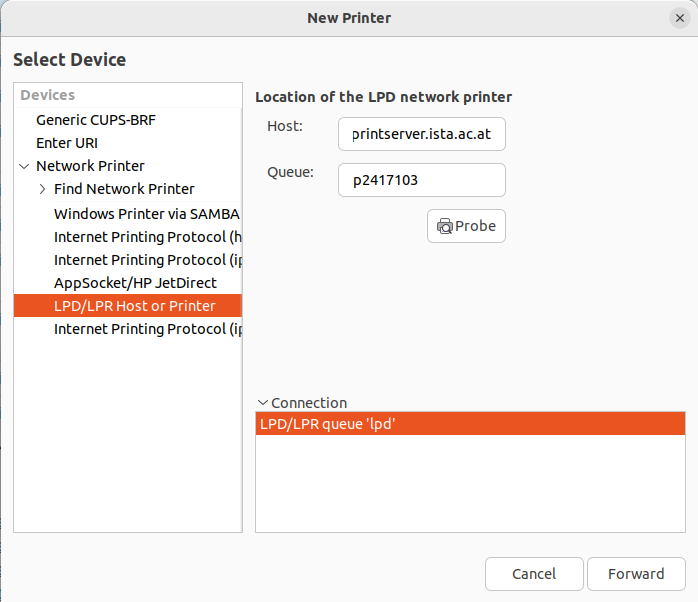
\includegraphics[width=.8\linewidth]{Figures/Printer_1.png}
        \caption{Step 3}
        \label{fig:sub1}
    \end{subfigure}
    \begin{subfigure}{.49\textwidth}
        \centering
        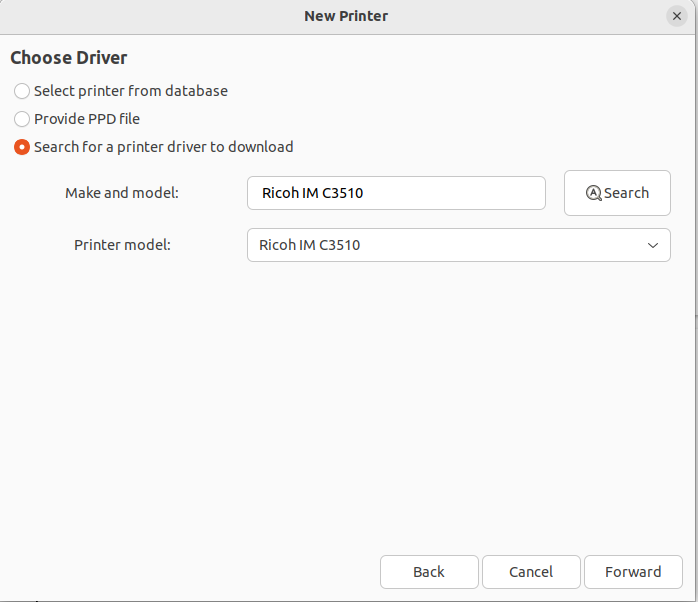
\includegraphics[width=.8\linewidth]{Figures/Printer_2.png}
        \caption{Step 4}
        \label{fig:sub2}
    \end{subfigure}
    \caption{Installing Printer}
    \label{fig:test}
\end{figure}




\end{document}
